\documentclass{beamer}
\usepackage{caption}
\usepackage{listings}
\AtBeginSection[]
{
  \begin{frame}
    \frametitle{Table of Contents}
    \tableofcontents[currentsection]
  \end{frame}
}
\usepackage[official]{eurosym}
% Remove the navigation buttons at the bottom right of each slide.
\setbeamertemplate{navigation symbols}{}
% Set bulletpoints to circles.
\setbeamertemplate{itemize items}[circle]


\title{Intro to Git}
\author{Netsoc}
% Remove the date.
\date{}
\begin{document}
\frame{\titlepage}

\section{Goals}
\begin{frame}
\frametitle{Goals}
\begin{itemize}
\item Show you the 10\% of Git that can do 90\% of the work
\item Slides \& practical demonstration
\item Answer questions
\end{itemize}
\end{frame}

\section{Git}
\begin{frame}
\frametitle{Git}
\begin{itemize}
\item Version Control System (VCS)
\begin{itemize}
\item Keep track of changes in files over time
\item Track who changed what, when
\item Help multiple people work on the same files at the same time
\item Detect and sometimes resolve conflicts automatically
\end{itemize}
\item Created by Linus Torvalds in 2005 for Linux Kernel development
\item Command-line program, available on Linux, Mac and Windows
\item Free and Open-Source
\item https://git-scm.com/
\end{itemize}
\end{frame}

\begin{frame}
\begin{figure}
\begin{center}
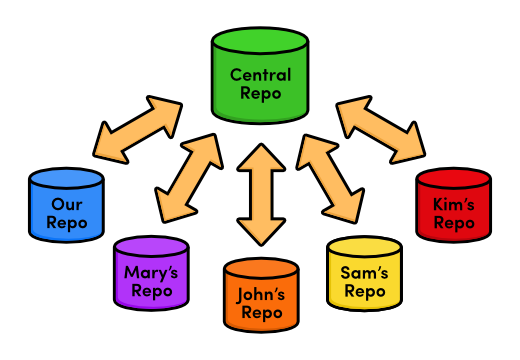
\includegraphics[scale=0.7]{centralised}
\caption{http://rypress.com/tutorials/git/media/8-7.png}
\end{center}
\end{figure}
\end{frame}

\section{Getting a repository}
\begin{frame}
\end{frame}

\section{Modifying your own repository}
\begin{frame}
\end{frame}

\section{Syncing your changes with other people}
\begin{frame}
\end{frame}

\section{Workflow}
\begin{frame}
\end{frame}

\end{document}

